\documentclass{beamer}
\usepackage{mathrsfs} %Pretty fonts
\usepackage{amsmath}
\usepackage{amssymb}
\usepackage{amsfonts}
\usepackage{amsthm}
\usepackage{bbm}
\usepackage{tikz}
\usetikzlibrary{arrows,shapes,positioning}
\usepackage{url} % insert Urls in bib
\usepackage[numbers]{natbib}
\bibliographystyle{plainnat}


\newtheorem{proposition}{Proposition}[section]

\mode<presentation>{\usetheme{Madrid}}
%%%% COMMANDS %%%%
% Real Numbers
\newcommand{\RNums}{\mathbb{R}}
% sigma-algebra
\newcommand{\salg}{\sigma\text{-algebra}}
% borel sigma-algebra
\newcommand{\borelsalg}{\mathscr{B}(\RNums)}
% Indicator function
\newcommand{\ind}{\mathbbm{1}}
% F: Sigma Algebra
\newcommand{\salgF}{\mathscr{F}}
% Probability P (P measure)
\newcommand{\Pm}{\mathbb{P}}
% Expectation's E
\newcommand{\E}{\mathbb{E}}
% Variance
\newcommand{\V}{\mathbb{V}}
% Continuous time stochastic process
\newcommand{\ctspr}{\{X_t\}_{t\geq 0}}
% Discrete time stochastic process
\newcommand{\dtspr}{\{X_n\}_{n\geq 0}}
% Insert only one number in the "align" environment
\newcommand\numberthis{\addtocounter{equation}{1}\tag{\theequation}}
% Measure Space
\newcommand{\MeasureSpace}[1]{(\Omega, \salgF, #1)}
% Proabability Space
\newcommand{\ProbSpace}{\MeasureSpace{\Pm}}
% Norm
\newcommand{\norm}[1]{\left\lVert#1\right\rVert}
% Inner Product
\newcommand{\innerprod}[2]{\langle #1, #2\rangle}


\title{Theoretical Grounds and Market Adaptations of Financial Fx and Interest Rate Options}
\author{Gerardo Dur\'an Mart\'in}
\institute{Universidad Marista}

\logo{\includegraphics[height=1.7cm]{UMA_logo}}

\begin{document}
%Generates the title page
\frame{\titlepage}

\begin{frame}
	\frametitle{Raison d'\^etre}
	\begin{enumerate}
		\item<1-> \textit{Plain vanilla} option pricing plays a big part in the derivatives' market;
		\item<2-> option pricing is mainly presented as a deeply esoteric subject that is too deep to delve into, or a complex one that requires a profound understanding in stochastic-calculus and analysis;
		\item<3-> to present the theory in a robust yet, accessible level for an undergraduate; and
		\item<4-> inquisitiveness.
	\end{enumerate}
\end{frame}
\AtBeginSection[]{
\begin{frame}
	\frametitle{Table of Contents}
	\tableofcontents[currentsection]
\end{frame}
}

\section{Financial Markets}

%% Market Assumptions
\begin{frame}
\frametitle{Some Important Definitions}

\only<1->{
\begin{definition}[Security]
	A security is an instrument that either represents ownership or that derives its value from a commodity.
\end{definition}
}

\only<2->{
\begin{definition}[Market]
	A market is the place where buyers meet sellers to exchange securities.
\end{definition}
}

\only<3->{
\begin{definition}[Arbitrage]
	We define an arbitrage as the probability of making a risk-free profit from a suitable market strategy.
	$$
		\Pm{(\text{Risk-free profit} > 0)} = 1
	$$
\end{definition}
}
\end{frame}


\begin{frame}
\frametitle{Market Assumptions}
\begin{itemize}
	\item Many buyers and sellers (liquidity);
	\item possible to lend and borrow at the same rate interest rate $r$;
	\item Market participants take advantage of arbitrage opportunity, thereby correcting any deviation from the actual value of any asset.
	\item All participants have the same information.
\end{itemize}
\end{frame}

%% Instruments
\begin{frame}
\frametitle{The Instruments}
	
	\begin{columns}[c]	
	
	\column{0.45\textwidth}
	\begin{itemize}
		\item <1-| alert@1> Bonds
		\item <2-| alert@2> Stocks
		\item <3-| alert@3> Foreign Exchange Currencies
		\item <4-| alert@4> Derivatives
	\end{itemize}
	
	\column{0.5\textwidth}
	\only<1>{
	A Bond is a debt obligation, its main function is to raise capital for the issuer of the bond. In turn, the buyer of the bond receives interest on the amount loaned.
	}
	\only<2>{
	A stock is a security that represents ownership on a fraction of a corporation. The return on the company for the owner of a stock is represented as a dividend.
	}
	\only<3>{
	``One country’s currency freely convertible in the foreign exchange market.'' (Kozikowski, 2013)
	}
	\only<4>{
	``[A derivative is] a financial instrument whose value depends on (or derives from) the values of other, more basic, underlying variables.'' (Hull, 2014)
	}
	\end{columns}
\end{frame}

%%Forwards
\begin{frame}
\frametitle{Derivatives: An Example}

	\begin{definition}[Forward]
		A forward is a derivative contract that gives the buyer both the right, and the obligation to to purchase a specified amount of the stock at some future time $T$, at a price $K$. The value of the forward today is 0.
	\end{definition}
	The payoff of the forward is $S_T - K$. What is the $K$ such that the contract has zero value today and has no possibility of arbitrage?
	
	\begin{figure}
	\includegraphics[width=0.45\textwidth]{../images/foward_payoff}
	\end{figure}
\end{frame}

\begin{frame}
\frametitle{Derivatives: An Example (cont'd)}
Assume a continuously compounded interest rate $r$, denote $S_t$ the value of the stock at time $t$. At $t=T$ the value of the forward is
$$
	S_T - K = 0
$$

By no arbitrage, the present value of the strategy is
$$
	S_0 - Ke^{-rT} = 0 \implies K = S_0e^{rT}
$$
Therefore, $S_0e^{rT}$ is the the value that guarantees no arbitrage.
\end{frame}

\begin{frame}
\frametitle{Derivatives: An Example (cont'd)}

(Why?)

Assume $K^\prime > K = S_0e^{rT}$. 
\begin{itemize}
	\item At $t=0$, borrow $S_0$; purchase the stock; and take a short position the forward contract.
	\item At $t=T$, receive $K^\prime$; give the forward; and repay $S_0e^{rT}$. Profit $K^\prime - S_0e^{rT}$.
\end{itemize}

The same can be said for $K^\prime < K$, by taking a long position.
\end{frame}

%%Option Pricing
\begin{frame}
\frametitle{Derivatives: Another Example}

\begin{definition}[European Call Option]
A European call option is a derivative contract that gives the buyer the right, but not the obligation to purchase a specified amount of stock at some future time $T$, at a price $K$.
\end{definition}

The payoff of the option is $\max\{S_T - K, 0\}$. What is the price of the option today that guarantees no arbitrage?

\begin{figure}
	\includegraphics[width=0.45\textwidth=]{../images/Call}
\end{figure}
\end{frame}

%%%%%%% Option Pricing: A Primer %%%%%%%
\section{A primer on Pricing}
\begin{frame}
\frametitle{One Step Binomial Model}
We assume a simple market consisting of a stock and a cash bond.
\begin{itemize}
	\item<1->{\textbf{The Stock}\\
	\begin{figure}[h!]
\centering
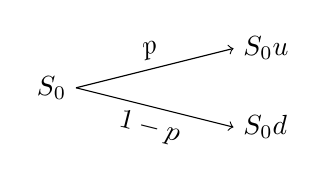
\begin{tikzpicture}
    \draw[->] (0,0) node[left]{$S_0$} --(2, 0.5) node[pos=0.5, sloped, above] {$p$};
    \node[right] at (2, 0.5) {$S_0u$};

    \draw[->] (0,0) --(2, -0.5) node[pos=0.5, sloped, below] {$1-p$};
    \node[right] at (2, -0.5) {$S_0d$};
\end{tikzpicture}
\end{figure}
Stock has value $S_0$ at outset. Between any two units of time, the stock can either go up by a factor $u$ (with probability $p$), or down by a factor $d$ (with probability $1-p$).
}
	\item<2>{\textbf{The Cash Bond}\\
	Represents the time value of money. $B_0$ invested at $t=0$ grows to $B_0e^{rT}$ one period thereafter.
	}
\end{itemize}
\end{frame}

\begin{frame}
	This simple market yields the possibility for a derivatives' market, i.e., there could be a payoff with price $f_0$ today that derives its value from the possible directions the stock may take: either $f_u$ if it goes up, or $f_d$ otherwise.
\begin{figure}
	
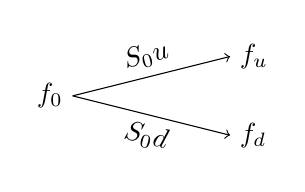
\begin{tikzpicture}
    \draw[->] (0,0) node[left]{$f_0$} --(2, 0.5) node[pos=0.5, sloped, above] {$S_0u$};
    \node[right] at (2, 0.5) {$f_u$};
    \draw[->] (0,0) --(2, -0.5) node[pos=0.5, sloped, below] {$S_0d$};
    \node[right] at (2, -0.5) {$f_d$};
\end{tikzpicture}
\end{figure}
\end{frame}

\begin{frame}
(Why?)
Consider the portfolio $(\phi, \psi)$ with $\phi$ number of stocks, and $\psi$ amount in the bank. The value of the portfolio at $t=0$ is
\[
    \phi S_0 + \psi B_0
\]
We derive a payoff $f$ contingent of the movement of the stock. At $t=\delta_t$ we have
\begin{align*}
    \phi S_0u + \psi B_0e^{r \delta_t} = f_u\\
    \phi S_0d + \psi B_0e^{r \delta_t} = f_d
\end{align*}

Yields,
\begin{align}
	\phi &= \frac{f_u - f_d}{S_0(u-d)}\\
	\psi &= e^{-r\delta_t} \frac{uf_d - df_u}{u -d}
\end{align}
\end{frame}

\begin{frame}
Therefore, buying the portfolio $(\phi, \psi)$ guarantees the payoff at $t=\delta_t$ (a risk-free strategy). Denote $\mathcal{V}$ the value of the portfolio at $t=0$.
\begin{equation} \label{eq:v_price_complete}
	\mathcal{V} = e^{-r\delta_t}\left[f_u \frac{e^{r\delta_t} - d}{u - d} + f_d \frac{u - e^{r\delta_t}}{u-d}\right].
\end{equation}

$\mathcal{V}$ is the cost of a risk-free strategy that guarantees the payoff. Furthermore, showing that $d < \exp{(r\delta_t)} < u$ proves that there exists no possibility of arbitrage.
\end{frame}

\begin{frame}
Denote
\begin{equation}
    q:= \frac{\exp{r\delta_t} - d}{u - d} \Longrightarrow 1-q = \frac{u - \exp{(r\delta_t)}}{u-d}.
\end{equation}

We rewrite (\ref{eq:v_price_complete}) as
\begin{equation} \label{eq:v_price}
    \mathcal{V} = \exp{(-r\delta_t)}[S_0u\cdot q + S_0d \cdot (1-q)] = \E_{\mathbb{Q}}[\mathcal{V}_{\delta_t}|\salgF_0].
\end{equation}
$\mathcal V$ is the discounted expectation under a probability measure $\mathbb Q$, and a martingale.
\end{frame}

%%%%%%% Stochastic Caluclus %%%%%%%
\section{Stochastic Calculus}

\begin{frame}
\frametitle{In Pursuance of a continuous-time model}
We pursue a continuous time model to price an option under such that replication (hedging) is possible and the condition of no arbitrage holds true. To do so we need
\begin{enumerate}
	\item A way to model the stock:
	\begin{itemize}
		\item a stochastic component, and
		\item a deterministic component.
	\end{itemize}
	\item tools to analyze the stock; and
	\item a way to hedge our position;
\end{enumerate}
\end{frame}

\begin{frame}
\frametitle{Brownian Motion}
We would like to have a stochastic process that models the dynamic of a stock. Any asset in the market should have a deterministic factor and a stochastic (noise) factor.
\begin{equation}
	\Delta S_t = \underbrace{\mu(t, S_t) \Delta t}_\text{Avg. rate of return} +
				 \underbrace{\sigma(t, S_t) \Delta W_t}_\text{Noise}
\end{equation}
\end{frame}

\begin{frame}
	In particular, we would like to model the following Stochastic differential equation:
	\begin{align*}
		\frac{dS_t}{S_t} &= \mu dt + \sigma dW_t
	\end{align*}
\begin{enumerate}
	\item What is its solution? (if any);
	\item how to model $dW_t$?;
	\item can the model be used to hedge any payoff?.
\end{enumerate}
\end{frame}

\begin{frame}
\frametitle{Noise Factor}
	It is logical to define this noise as a Brownian motion:
	\begin{definition}[Brownian Motion]
	\begin{itemize}
		\item $W_0 = 0$;
		\item The trajectories are continuous; 
		\item The process has independent increments; and
		\item $W_t - W_s \sim N(0, \sigma^2(t - s); \ 0 \leq s \leq t$.
	\end{itemize}
	\end{definition}
	
\begin{table}
\centering
\label{table:bm-property}
\begin{tabular}{l|ll}
       & $dW_t$ & $dt$ \\
       \hline
$dW_t$ & $dt$   & 0    \\
$dt$   & 0      & 0   
\end{tabular}
\caption{Dynamics of the Brownian Motion in $L_2$}
\end{table}
\end{frame}

\begin{frame}
\frametitle{Dynamics}
\framesubtitle{What if the stock moves in continuous time?}
Let $W(\cdot)$ an n-dimensional Brownian motion process over $\ProbSpace$ and let $\mathscr{G}$, a family of $\salg$s where
	\begin{enumerate}
		\item $\mathscr{G}(s) \subseteq \mathscr{G}(t)$ for all $0\leq s \leq t$;
		\item For all $t, h > 0$, $W_{t+h} - W_t$ is independent of $\mathscr{G}(t)$.
	\end{enumerate}
	We will be working on a family $\Nhatfam{0}{T}$ of functions such that
	\begin{definition}[$\Nhatfam{0}{T}$]
	\begin{enumerate}
		\item $(t, \omega) \to f(t, \omega):[0, \infty]\times\Omega \to \RNums$ is $\borelsalg\times\salgF$ measurable;
		\item $\int_0^t f^2(s) ds < \infty$ a.s.; and
		\item $f(\cdot, \omega)$ is independent of $\mathscr{G}(\cdot)$.
	\end{enumerate}
\end{definition}
\end{frame}

\begin{frame}
	\frametitle{The It\^o Integral}
	We define a discrete-time It\^o Integral over $\Nhatfam{0}{T}$ as the sum of simple processes $f_n$ such that
	\begin{equation}
		\int_0^T f_n(t) dW_t := \sum_{i=0}^{n-1}f(t_i) \Delta W_i
	\end{equation}
	Where $\Delta W_i := W_{i+1} - W_i$
\end{frame}

\begin{frame}
	\begin{figure}[hbt]
  \includegraphics[width=0.9\textwidth]{../images/simple_process}
  \caption{Simple Process}
\end{figure}
\end{frame}

\begin{frame}
	\frametitle{The It\^o Integral}
	More generally, 
	\begin{definition}
	define It\^o integral $\int_0^t fdW_t$ for $f\in \Nhatfam{0}{T}$ over a probability space $\ProbSpace$ as the limit (in probability) of of simple functions $f_n$ such that
		\begin{equation}
		\lim_{n\to \infty} \Pm\left(\left\{\omega: \int_0^t f_n(t,\omega)dW_t - \int_0^t f(t,\omega)dW_t > \epsilon\right\} \right) = 0
	\end{equation}
	\end{definition}
\end{frame}

\begin{frame}
\frametitle{It\^o Process}
\begin{definition}[\textbf{It\^o Process}]
	let $W_t$ a standard Brownian motion on $\ProbSpace$. We define the It\^o process $X(t)$ over $\ProbSpace$ as
	\begin{equation}
		X(t) := \int_0^t\mu(s,\omega) ds  + \int_0^t\sigma(s,\omega) dW_s.
	\end{equation}
		
	Where
	\begin{enumerate}
		\item $\int_0^t \mu(s,\omega) ds < \infty$; and
		\item $\sigma(s,\omega) \in \Nhatfam{0}{T}$.
	\end{enumerate}
\end{definition}

The It\^o process is also represented in differential form:
\begin{equation*}
	dX(t) = \mu(t,\omega) dt + \sigma(t,\omega) dW_t
\end{equation*}
\end{frame}

\begin{frame}
\begin{theorem}[\textbf{It\^o's Formula}]\label{th:itos_formula}
	Let $X(t)$ be an It\^o process of the form
	\[
		dX(t) = \mu(t, \omega) dt + \sigma(t, \omega) dW_t,
	\]
	and $g(t, \omega) \in C^2([0, \infty]\times\RNums)$. Then,
	\begin{equation*}
		Y(t) := g(t, X_t)
	\end{equation*}
	is also an It\^o Process where
	
	\begin{equation*}
		dY(t) = \partialwrt{g}{t}(t, X(t)) dt + \partialwrt{g}{x}(t, X(t)) \left(dX(t)\right) + \frac{1}{2}\partialwrt[2]{g}{x} (t, X(t)) \left(dX(t)\right)^2
	\end{equation*}	
\end{theorem}	
\end{frame}

\begin{frame}
In particular, It\^o's formula is the tool we need to get to a closed form for an asset with dynamics
	\[
	\frac{dS_t}{S_t} = \mu dt + \sigma dW_t \Rightarrow S_t = S_0e^{\left(\mu - \frac{1}{2}\sigma^2\right) t + \sigma\int_0^t dW_s}
	\]
	
\begin{figure}[hbt]
  \includegraphics[width=0.7\textwidth]{../images/asset_sde}
  \caption{SDE with $\sigma=0$ and $\sigma=0.2$}
\end{figure}
\end{frame}

\begin{frame}
	\frametitle{Black-Scholes}
	Consider a market with two securities
	\begin{align*}
	dB_t &= r B_t dt \\
	dS_t &= S_t(\mu dt + \sigma dW_t)
	\end{align*}
	
\begin{theorem}[\textbf{Black-Scholes Equation}]
	Consider a European claim $g(\omega)$ at time $T$. The price of the claim at time $0\leq t\leq T$ is given by $C(t,S_t)$, where $C$ is the solution to the partial differential equation
	
	\begin{equation}\label{eq:black-scholes-formula}
		\partialwrt{C}{t} + \frac{1}{2}\sigma^2S^2\partialwrt[2]{C}{S} + rS\partialwrt{C}{S} - rC = 0,
	\end{equation}

with final boundary condition $C(T) = g(T, S_T)$.
\end{theorem}
\end{frame}

\begin{frame}
\frametitle{Black-Scholes Formula proof (sketch)}
	By It\^o`s formula we have

\begin{equation}
	dC(t, S_t) = \left(C_t + \mu S_t C_s + \frac{1}{2}(S_t\sigma)^2C_{ss} \right) dt  + S_t\sigma C_s dW_t \label{eqproof:claim_bs}
\end{equation}

And, for the replicating portfolio, let $\pi(t)$ be the total amount of cash invested in $S_t$ then,
\begin{align}
	d\valueProcess{t} &= \theta_0(t)dB_t  + \theta_1 dS_t \nonumber \\
					&= [r\valueProcess{t} + (\mu - r) \pi(t)] dt + \sigma\pi(t) dW_t \label{eqproof:portfolio_bs}
\end{align}
\end{frame}

\begin{frame}
\frametitle{Black-Scholes Formula proof (sketch) cont'd}
	Having a replicating portfolio $V^\theta$, a claim $C$ to honor at time $T$, we need	
\begin{equation}
	\valueProcess{T} = g(S_T) = C(T, S_T).
\end{equation}

We can rewrite this last equation in differential form, and considering the law of one price as:
\[
	d\valueProcess{t} = dC(t, S_t) \ \forall \ t \in [0,T].
\]

Wich yields
\begin{equation}
  C_t + \frac{1}{2}(S_t\sigma)^2C_{ss} + rS_t C_s - rC = 0
\end{equation}
\end{frame}


\begin{frame}
\frametitle{Markets}

We can reach to a closed-form solution in a similar-route
\begin{definition}
A market $X(t) = \{X_i(t)\}_{i=0}^n$ is an $\salgF^{(m)}_t$-adapted $n+1$ It\^o Process where
\begin{equation}
	dX_0 = r(t,\omega) X_0(t) dt; \ X(0) = 1; \label{eq:safe_investment}
\end{equation} 

and
\begin{equation}
	dX_i = \mu_i(t,\omega) dt + \sum_{j=1}^{m}\sigma_{ij}(t,\omega)dW_j(t) \label{eq:risky_asset}.
\end{equation}
\end{definition}
\end{frame}

\begin{frame}
\begin{definition}[\textbf{Portfolio}]
A portfolio $\theta(t)$ in the market $\market$ is an ($n+1$)-dimensional $(t,\omega)$-measurable and $\salgF_t^{(m)}$-adapted stochastic process
\begin{equation}
	\theta(t,\omega) = \{\theta_{i}(t,\omega)\}_{i=0}^{n} \ \forall \ t\in[0, T].
\end{equation}
\end{definition}

\begin{definition}[\textbf{The value process}]
The value at time $t$ for the portfolio $\theta$ is defined as
\begin{equation}
	V(t) = \innerprod{\theta(t)}{X(t)} = \theta(t) \cdot X(t)
\end{equation}
\end{definition}
\end{frame}

\begin{frame}
\begin{definition}[\textbf{Self-financing portfolio}]\label{def:self-financing-portfolio}
	The portfolio $\theta(t)$ is said to be self-financing if
	\begin{equation*}
	\int_0^T\underbrace{\{|\theta_0r(s)X_0(s) + \sum_{i=1}^{n}\theta_i(s)\mu(s)|}_{\text{Integrability ($L_1$) condition}} + \sum_{j=1}^m\underbrace{\left[\sum_{i=1}^n\theta_i(s)\sigma_{ij}(s)\right]^2}_{\text{$\Nhatfam{0}{T}$ condition}}\} ds < \infty,
	\end{equation*}
and 
\begin{equation*}
  dV(t) = \innerprod{\theta(t)}{dX(t)} \iff V(t) = V(0)  + \int_0^t \theta(s) dX(s).
\end{equation*}

\end{definition}
\end{frame}

\begin{frame}
	\begin{definition}[\textbf{Claims}]
\begin{enumerate}
	\item A contigent claim $T$ is a lower bounded $\salgF_t^{(m)}$-measurable random variable $C(\omega)$;
	\item A claim $C(\omega)$ is said to be attainable if there exists an admissible portfolio $\theta(t)$ and $z\in\RNums$ such that
	\[
		C(\omega) = V_z^{\theta}(T) := z + \int_0^T \theta(t)dX(t) \text{a.s. and,}
	\]
	
	\begin{equation}
		\valueProcessNorm{T}	 = z + \int_0^t \nu(s)\sum_{i=1}^{n}\theta_i(s)\sigma_i(s) dW^\Qm_s \ \forall \ 0 \leq t \leq T
	\end{equation} 
	is a $\Qm$-martingale. If such $\theta$ exists, it is called a replicating portfolio.
	\item A market $\market$ is said to be complete if every bounded claim at time $T$ is attainable.
\end{enumerate}
\end{definition}
\end{frame}

\begin{frame}
In what follows, we will assume $u(t,\omega) \in \Nhatfam{0}{T}$ such that
\begin{equation}\label{eq:condition_change_measure}
	\sigma(t,\omega) u(t,\omega) = \mu(t,\omega) - r(t,\omega) X_t,
\end{equation}
and let $\Qm$, and $W_t^\Qm$ such that
\begin{align}
  d\Qm = e^{-\left(\int_0^t u(t,\omega) dW_t + \frac{1}{2}\int_0^T u^2(t,\omega) dt\right)} d\Pm \label{eq:emmq} \\
  W^\Qm_t := \int_0^t (s,\omega) ds + W_t
\end{align}

Then,
\begin{itemize}
	\item There exists an equivalent martingale measure;
	\item therefore, no arbitrage;
	\item which implies a complete market;
	\item for which we conclude that there exists a fair price $c$ such that
	\[
		c = \ExpMeasure{\Qm}{\nu(T)g(S_t)}
	\]
\end{itemize}
\end{frame}

\begin{frame}
Since we have
\begin{align*}
	dS_t =  S_t(\mu dt + \sigma dW_t); \ \text{under $\Pm$}\\
	dS_t =  S_t(r dt + \sigma dW_t); \ \text{under $\Qm$}
\end{align*}
We compute a risk-free price for the claim $C$ at $t=0$ as:
\begin{align*}
	c &= \ExpMeasure{\Qm}{\nu(T)g(S_t)}\\
	 &= \nu(T)\ExpMeasure{\Qm}{g(S_0e^{\left(\mu - \frac{1}{2}\sigma^2\right) t + \sigma\int_0^t dW_s})}
\end{align*}
\end{frame}

\begin{frame}
\frametitle{The case of a call European option}
	For a call European option we have:
	\begin{align}
	c &= \nu(T)\ExpMeasure{\Qm}{\max\{S_0e^{\left(\mu - \frac{1}{2}\sigma^2\right) t + \sigma\int_0^t dW_s},0\}}\\
		&= S_0N(d_+) - Ke^{-rT}N(d_-).
	\end{align}
	With,
\begin{equation}
d_\pm = \frac{1}{\sigma \sqrt T}\left(\log \frac{S_0}{K} \pm (r - \frac{1}{2}\sigma^2)T\right)  
\end{equation}
\end{frame}

\begin{frame}
\frametitle{What about the Black-Scholes PDE?}
It turns out that the Feynman-Kac formula relates the conditional risk-neutral expectation of the claim and the Black-Scholes PDE
\begin{theorem}[\textbf{Feynman-Kac}]
	Consider the following partial differential equation
	\begin{equation*}
		\partialwrt{C}{t}{(t,x)}	 + \mu(t, x)\partialwrt{C}{x}{(t,x)} + \frac{1}{2}\sigma^2(t,x)\partialwrt[2]{C}{x}{(t,x)}  - V(t,x)C(t,x) + f(x,t) = 0 \label{eq:feynman_kac_pde}.
	\end{equation*}
	Defined for $x\in\RNums$, $t\in[0,T]$ and subject to the final boundary condition $C(T, X_T) = P(X_T)$. Then, $C(x,t)$ can be written as the following conditional expectation
	\begin{equation}
	C(t, x) = \Exp{\int_t^Te^{-\int_t^r V(X_\tau, \tau) d\tau} f(X_r, r) dr + e^{-\int_t^TV(\tau, X_\tau) d\tau} P(X_T)| \salgF_t}.
	\end{equation}

Where $X_t$ is the It\^o process $dX_t = \mu(t,x) dt + \sigma(t, X_t) dW_t$.
\end{theorem}

\end{frame}

%\nocite{*}
%\bibliography{../misc/ref}

\end{document}